\documentclass[border=5px]{standalone}
\def\pgfsysdriver{pgfsys-pdftex.def}
\usepackage[usenames,dvipsnames,svgnames,x11names,table]{xcolor}
\usepackage{tikz}
\usetikzlibrary{arrows,positioning,automata,shadows,fit,shapes,patterns,fadings}
\usetikzlibrary{shadows}
\begin{document}
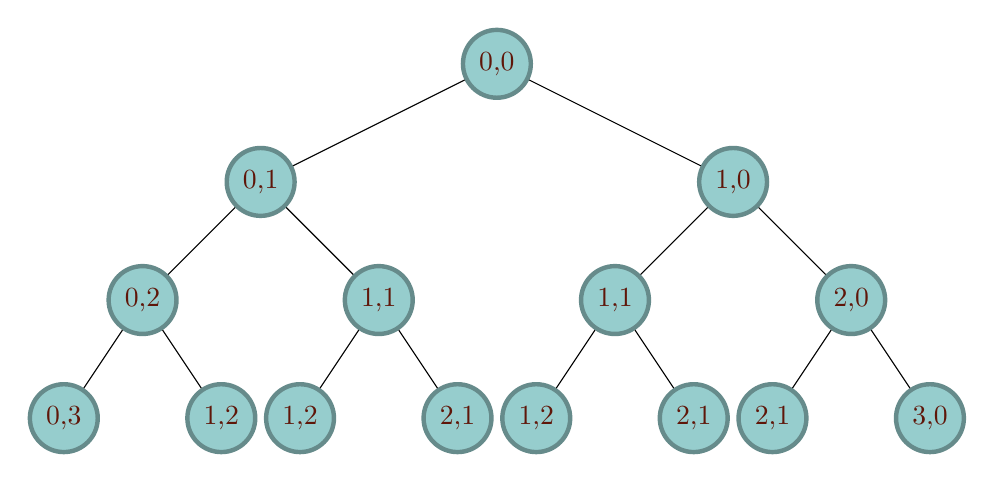
\begin{tikzpicture}
\tikzstyle{every node}=[circle,fill=PaleTurquoise3,draw=PaleTurquoise4,ultra thick,text=Sepia];
\tikzstyle{level 1}=[sibling distance=60mm];
\tikzstyle{level 2}=[sibling distance=30mm];
\tikzstyle{level 3}=[sibling distance=20mm];
\node {0,0}
child {node {0,1}
    child {node {0,2}
        child {node {0,3}}
        child {node {1,2}}
    }
child {node {1,1}
    child {node {1,2}}
    child {node {2,1}}
    }
}
child {node {1,0}
        child {node {1,1}
        child {node {1,2}}
        child {node {2,1}}
    }
child {node {2,0}
        child{node{2,1}}
        child{node{3,0}}
}
}; 
\end{tikzpicture}
\end{document}
